\section{Preliminaries}\label{sec:prelim}

\subsection{Notations}

A multi-turn dialogue prefix of length $k$ is $\mathcal{D}_k=\{(q_1,a_1),\ldots,(q_k,a_k)\}$, where $q_t$ is the user query at turn $t$ and $a_t$ is the model response. We write $F$ for the original model, a proprietary black-box LLM as is common in machine-learning-as-a-service (MLaaS), and $G$ for the small surrogate. The textual response of model $M\in\{F,G\}$ at turn $t$ is $a_t^M$. Let $f_M(\cdot)$ map an input sequence to the hidden space, so that $\mathbf{h}_t=f_M(q_{\le t})\in\mathbb{R}^d$ is the hidden state at turn $t$; the first $k$ hidden states $\mathcal{H}_k=\{\mathbf{h}_1,\ldots,\mathbf{h}_k\}$ induce a local region $\mathcal{M}_k^M\subset\mathbb{R}^d$. A soft prompt of length $L$ is a matrix $\mathbf{P}\in\mathbb{R}^{L\times d}$. Appendix~\ref{sec:notation} lists all symbols.

\subsection{Exploring Token--Turn Patterns in Multi-Turn LLM Dialogues}
\label{sec:long_tail}

Standard serving processes each new request together with the entire history, so the cost of a turn grows with the length of the conversation. The amount of \emph{new} information in a turn, however, need not grow at all. We therefore first study token usage across turns.


We consider four representative settings: \textit{ShareGPT}~\citep{chen2024sharegpt4v} for open-ended human--LLM chat, \textit{ReMeDi}~\citep{yan2022remedi} for doctor--patient consultation, \textit{Craigslist Bargain}~\citep{he2018decoupling} for negotiation, and \textit{Multi-Character}~\citep{agentlans_multi-character_dialogue_2024} for multi-party role-play. Together they cover different speaker roles, task goals, and interaction structures. For each dataset, we compute the average token count at turn \(t\) and normalize it by the average of Turn~1.

\begin{wrapfigure}[13]{r}{0.42\textwidth}
  \vspace{-11pt}
  \centering
  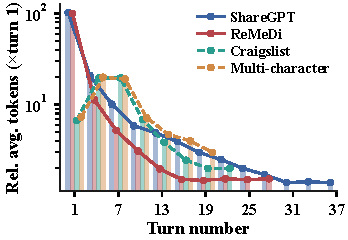
\includegraphics[width=0.419\textwidth]{figure/long_tail.pdf}
  \vspace{-18pt}
  \caption{Average token count per turn, normalized by Turn~1, on four dialogue datasets: usage drops after the early turns and forms a long tail.}
  \vspace{-11pt}
  \label{fig:longtail-token-decay}
\end{wrapfigure}
Figure~\ref{fig:longtail-token-decay} shows a consistent long-tail pattern. Early turns are token-heavy: they introduce the task, the topic, the constraints, and the speaker's intent. Later turns are much shorter and settle at a low, stable level. Shorter does not mean independent. Many later turns read as local updates to a dialogue state that has already been established, so the marginal new input shrinks while standard serving keeps re-processing the full prefix. This mismatch motivates an adaptive strategy: let the original model establish the early dialogue state, and hand subsequent turns to a cheaper surrogate for as long as they stay within that state, instead of recomputing the full history.

\subsection{Local Manifold Approximation for Multi-Turn Dialogues}

The long-tail pattern creates an opportunity for surrogate serving, but a naive substitution is unreliable. A later turn is short precisely because much of its meaning is supplied by the preceding dialogue, so a surrogate that is not aligned with the original model under that prefix produces fluent responses that quietly drift from the intended context.

We describe this challenge through a local manifold view. Given a prefix \(\mathcal{D}_{k}\), the original model \(F\) and the surrogate \(G\) each induce a local region in their contextual representation space, and this region captures the current topic, constraints, style, and task state. The goal is to make the surrogate's region match that of the original model under the same prefix.

\begin{problem}[Local Manifold Approximation for Multi-Turn Interactions]
Given a dialogue prefix \(\mathcal{D}_{k}\) and an original model \(F\), learn a surrogate model \(G\in\mathcal{G}\) whose local representation region matches that of \(F\) under the same prefix:
\[
\min_{G\in\mathcal{G}}
\mathrm{dist}\!\left(
\mathcal{M}^{G}_{k}(\mathcal{D}_{k}),
\mathcal{M}^{F}_{k}(\mathcal{D}_{k})
\right),
\]
where \(\mathcal{M}^{F}_{k}(\mathcal{D}_{k})\) and \(\mathcal{M}^{G}_{k}(\mathcal{D}_{k})\) denote the local representation regions induced by the prefix, and \(\mathrm{dist}(\cdot,\cdot)\) measures their discrepancy.
\end{problem}

This formulation leads directly to SOMA. The early turns are used to expose where the surrogate disagrees with the original model within the current dialogue state, and these locally informative examples are then used to adapt the surrogate. After adaptation, the surrogate serves later turns only while the dialogue remains close to the learned region; when the conversation drifts, the system returns to the original model and refreshes the local state.
